\documentclass[letterpaper,10pt]{article}

\usepackage{titling}
\usepackage{listings}
\usepackage{url}
\usepackage{setspace}
\usepackage{subfig}
\usepackage{sectsty}
\usepackage{pdfpages}
\usepackage{colortbl}
\usepackage{multirow}
\usepackage{relsize}
\usepackage{amsmath}
\usepackage{fancyvrb}
\usepackage{amsmath,amssymb,amsthm,graphicx,xspace}
\usepackage[titlenotnumbered,noend,noline]{algorithm2e}
\usepackage[compact]{titlesec}
\usepackage{paratype} 
\usepackage[T1]{fontenc}
\usepackage{tikz}
\usetikzlibrary{arrows,automata,shapes,trees,matrix,chains,scopes,positioning,calc}
\tikzstyle{block} = [rectangle, draw, fill=blue!20, 
    text width=2.5em, text centered, rounded corners, minimum height=2em]
\tikzstyle{bw} = [rectangle, draw, fill=blue!20, 
    text width=4em, text centered, rounded corners, minimum height=2em]

\definecolor{namerow}{cmyk}{.40,.40,.40,.40}
\definecolor{namecol}{cmyk}{.40,.40,.40,.40}

\let\LaTeXtitle\title
\renewcommand{\title}[1]{\LaTeXtitle{\textsf{#1}}}


\newcommand{\handout}[5]{
  \noindent
  \begin{center}
  \framebox{
    \vbox{
      \hbox to 5.78in { {\bf ECE254: Operating Systems and Systems Programming } \hfill #2 }
      \vspace{4mm}
      \hbox to 5.78in { {\Large \hfill #4  \hfill} }
      \vspace{2mm}
      \hbox to 5.78in { {\em #3 \hfill} }
    }
  }
  \end{center}
  \vspace*{4mm}
}

\newcommand{\lecture}[3]{\handout{#1}{#2}{#3}{Lecture #1}}
\newcommand{\tuple}[1]{\ensuremath{\left\langle #1 \right\rangle}\xspace}

\addtolength{\oddsidemargin}{-1.000in}
\addtolength{\evensidemargin}{-0.500in}
\addtolength{\textwidth}{2.0in}
\addtolength{\topmargin}{-1.000in}
\addtolength{\textheight}{1.75in}
\addtolength{\parskip}{\baselineskip}
\setlength{\parindent}{0in}
\renewcommand{\baselinestretch}{1.5}
\newcommand{\term}{Spring 2015}

\singlespace


\begin{document}

\lecture{ 21 --- Memory: Segmentation and Paging }{\term}{Jeff Zarnett}

\section*{Memory Segmentation}

Though you've been repeatedly told that memory is a linear array of bytes, you have also likely been told that there's the stack and the heap, libraries and instructions. Both of these are true; they are simply views of memory at two different levels of abstraction. Each of the elements such as the stack, the heap, the standard C library, et cetera, are known as \textit{segments}.

Programmers do not necessarily give much thought to whether variables are allocated on the stack or the heap, or where program instructions appear in memory. In many cases it does not matter, though C programmers are well advised to know the difference.

A full program has a collection of segments, each of which may be different lengths. Normally the compiler is responsible for constructing the various segments; perhaps one for each of the following~\cite{osc}:

\begin{enumerate}
	\item The code (instructions).
	\item Global variables.
	\item The heap.
	\item The stack (one per thread).
	\item The standard C library.
\end{enumerate}

From the programmer's perspective, memory may simply be various blocks, as below:

\begin{center}
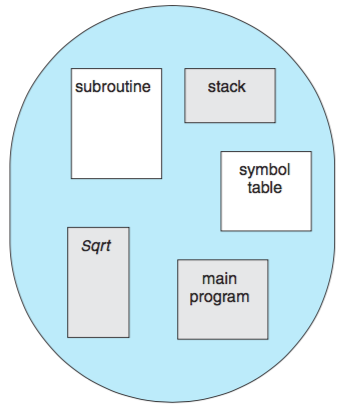
\includegraphics[width=0.25\textwidth]{images/segments.png}\\
One way programmers might look at memory~\cite{osc}.
\end{center}

Rather than thinking about memory as just a pure address, we can think of it as a tuple: \textit{$<$segment, offset$>$}. Given that, we need an implementation to map these tuples into memory addresses. The mapping has a segment table; each entry in the table contains two values: the base (starting address of the segment) and the limit (the length of the segment). So there will be some addition involved as well as a comparison to see if the address lies within that range. As is typically the case, memory accesses are such a common operation that we will need another rescue from the hardware folks to make this not painfully slow.

\begin{center}
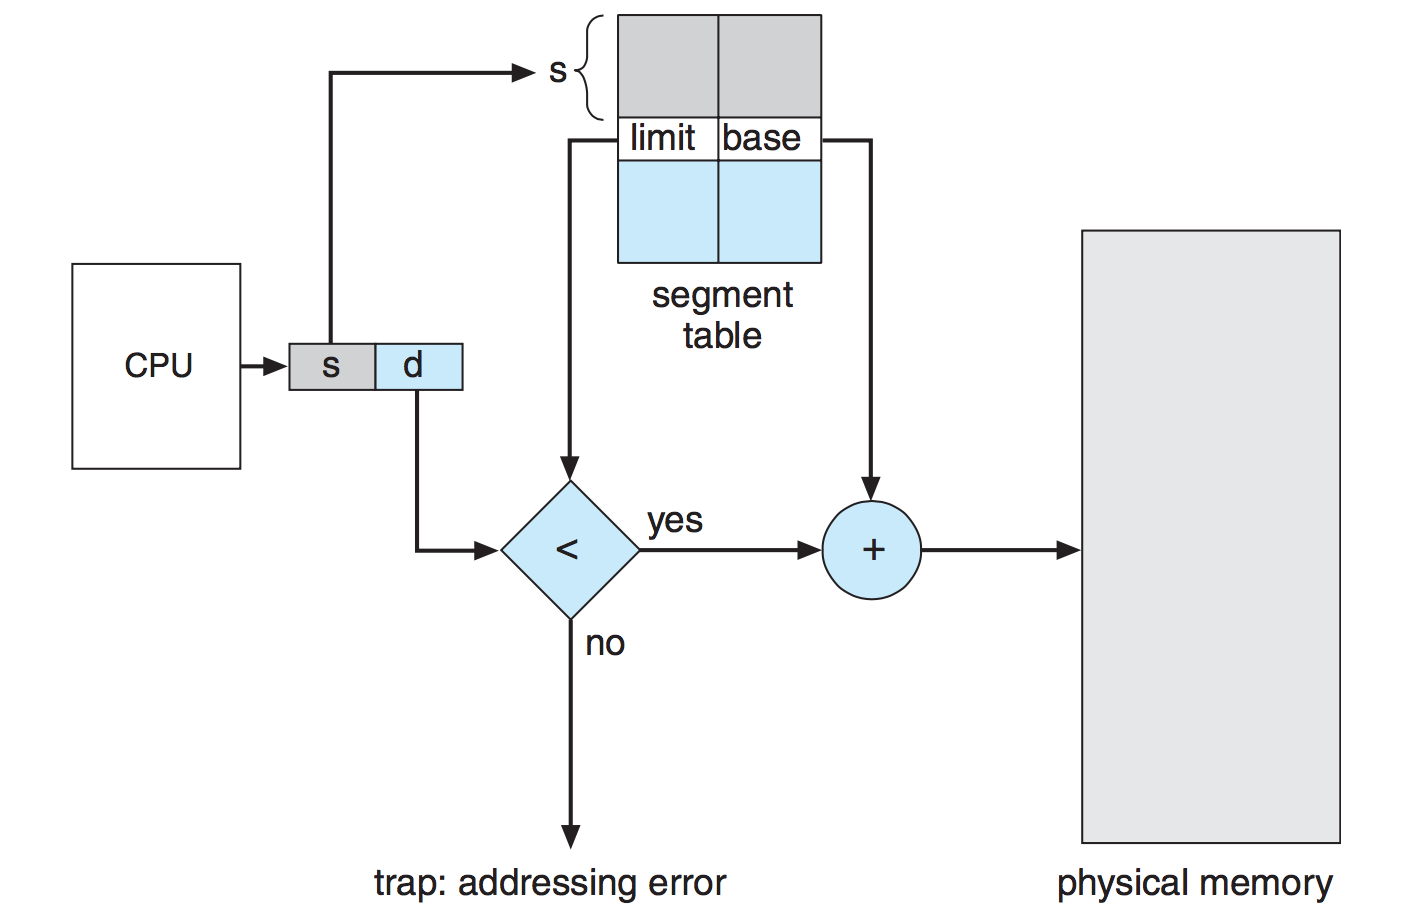
\includegraphics[width=0.75\textwidth]{images/segmentation-hardware.png}\\
Segmentation hardware~\cite{osc}.
\end{center}

With segmentation, memory need longer be contiguous; we can allocate different parts of the program in different segments; different segments can be located in different areas of memory.

\section*{Paging}
Fixed and variable sized partitions suffer from fragmentation, whether external or internal. Let us divide memory up into small, fixed-size chunks of equal size, called \textit{frames}. Each process's memory is divided up into chunks the same size as a frame, called \textit{pages}. Then a page can be assigned to a frame. A frame may be empty or may have exactly one page in it. 

Imagine, as an analogy, a simple picture frame. The frame may be empty or it may contain a picture. If the picture frame is empty, all that is necessary is to put a picture in it. To put in a different picture, you would first need to take out the picture that is already there. Taking out the picture to empty the frame is allowed, too. A picture is always aligned so that it is completely in one frame; not half in and half out. Now expand this scheme by having a very long row of picture frames, each of which can contain one picture at a time, at most, and a picture can be in at most one frame at a time. 

When a process starts, it is loaded into memory, and has some initial memory requirements (e.g., the stack and global variables), so it will require some number of pages. The number of pages can and will change over time as memory is allocated and freed. A process may also be swapped out to disk, but to run it will need to be swapped back in. Either way, a process will take up a certain number of pages in memory at any given time.

Pages provide the benefit of separating the logical address from the physical address: programmers may pretend the address space of the computer is $2^{64}$ bytes rather than however many GB of memory are in the physical machine. 

Consider the diagram below, in which there are 15 free frames initially. Then we load process $A$, which consists of 4 frames; then process $B$ with 3 frames, $C$ with another 3 frames. Eventually, $B$ is swapped out (put back on disk) and $D$ is loaded. Process $D$ has five frames, but the frames do not have to be contiguous (and although they are shown in order, they do not necessarily have to be).

\begin{center}
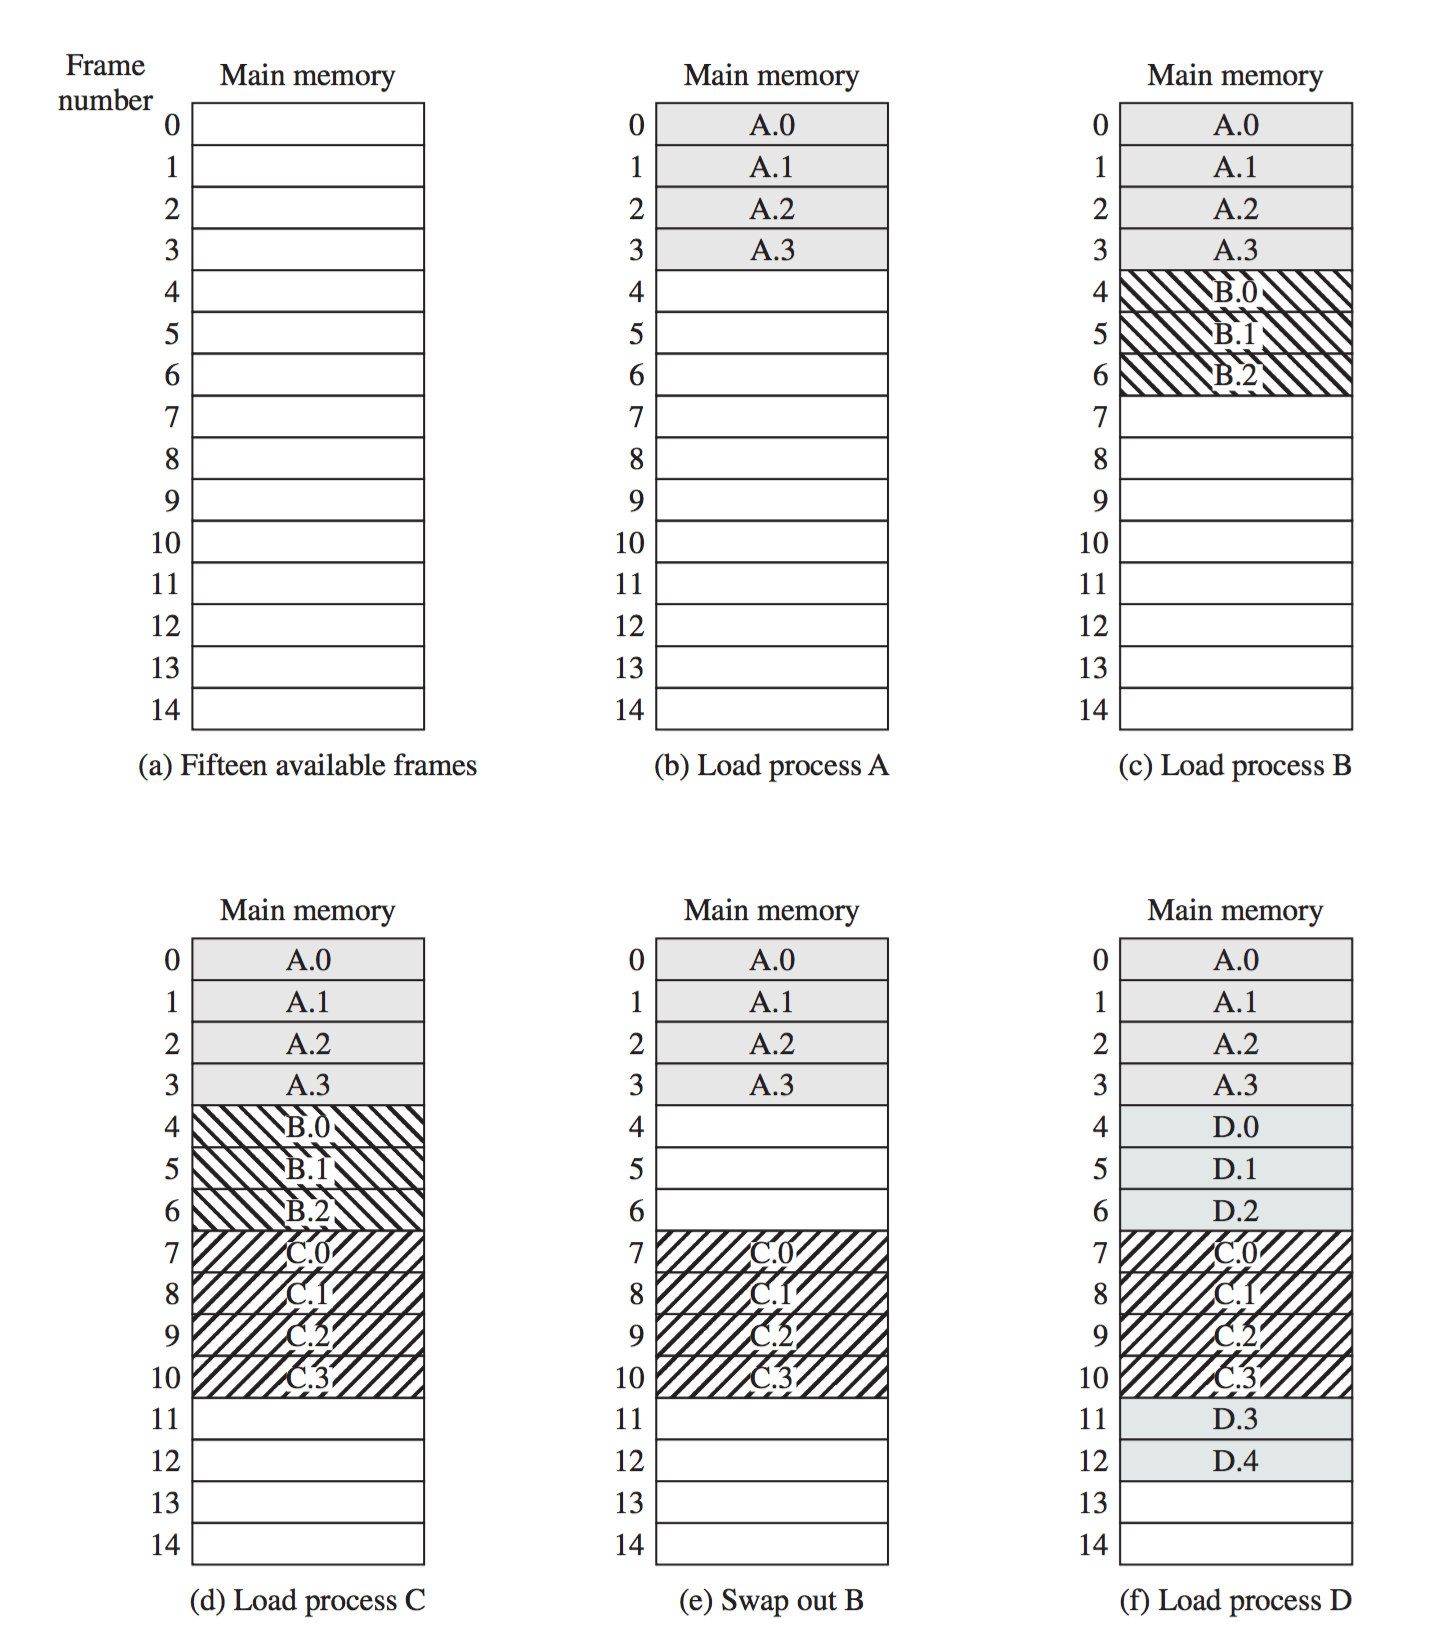
\includegraphics[width=0.75\textwidth]{images/loading-pages.png}\\
Assignment of process pages into free frames~\cite{osi}.
\end{center}

Now that we have multiple segments for each process and they are no longer contiguous, it is insufficient to have a base address and a limit. Now instead, each process needs a page table, to keep track of which pages are located where in memory. A list of free frames is also necessary. See the diagram below:

\begin{center}
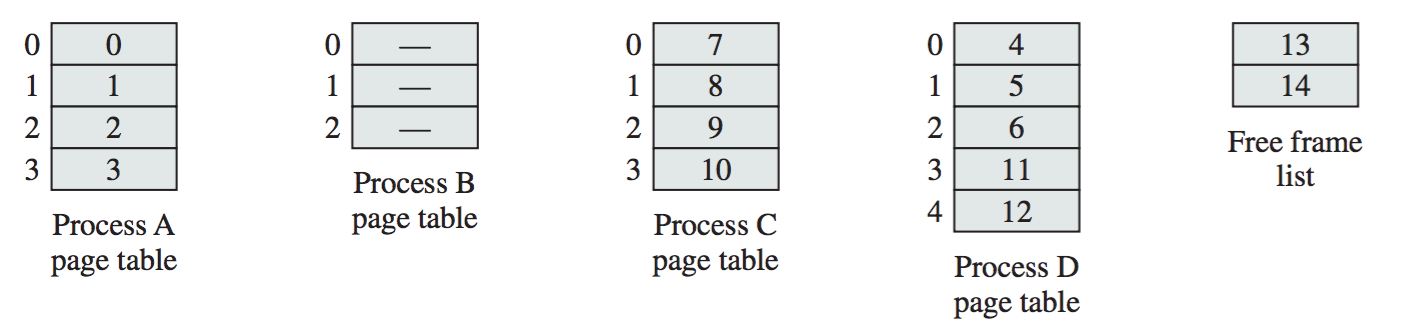
\includegraphics[width=0.75\textwidth]{images/page-tables.png}\\
The page tables as of (f) in the previous diagram~\cite{osi}.
\end{center}

The page table is used to map logical memory to physical memory, as in the diagram below:

\begin{center}
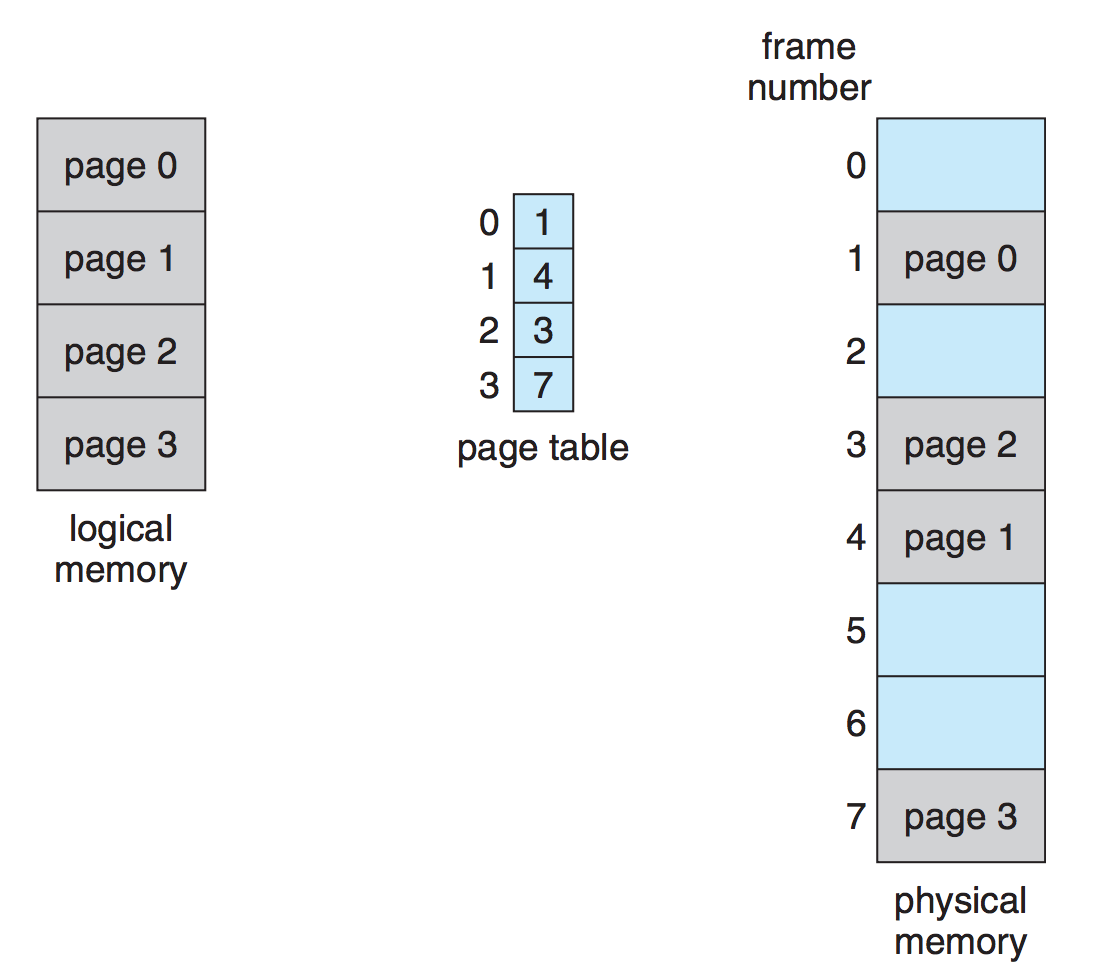
\includegraphics[width=0.5\textwidth]{images/page-table-mapping.png}\\
Mapping of logical memory to physical memory via the page table~\cite{osc}.
\end{center}

For convenience, page size is usually a power of 2 (and the actual value is determined by hardware). The selection of a power of 2 makes translating a logical address into a tuple of the page number and offset easy. If the logical address space has size $2^{m}$ and the page size is $2^{n}$ bytes, $n$ obviously smaller than $m$, then the high order $m - n$ bits of the logical address are the page number and the lower $n$ bits are the page offset~\cite{osc}. 

External fragmentation is eliminated as a problem in this scheme, because pages are all the same size. That also means that compaction is not an issue. Compaction, when it's possible, is painful enough in memory; it is excruciating to do on disk. It is therefore desirable to avoid it entirely. We accept some internal fragmentation because a process gets a whole page at a time. 

But how much internal fragmentation do we have to live with? Not very much. If the memory required aligns perfectly with a multiple of the page size, then no memory is wasted. If a new memory allocation comes in, then a new page is allocated and added to the logical memory space of the process. The last frame, however, may not be completely full. In the worst case scenario, a full page less one byte is wasted. However, internal fragmentation of one page is not very much in the grand scheme of things.

How big should page sizes be? If they are smaller, then less memory is wasted in internal fragmentation. However, having a large number of pages introduces a lot of overhead. The size of pages has tended to grow along with the size of main memory in computers~\cite{osc}. The key factor is actually disk: the disk operates on a certain block size and it is most efficient for the size of a page to be equal to a disk read/write size. That way when a page is to be swapped into or out of memory, it can be done in a single disk read or write. In a typical modern system, pages are 4~KB, but they can be bigger.

Now we finally have a good answer to why the application developer can treat memory as if it is infinitely large and unshared. The program is scattered across physical memory, but appears to the application developer and running application as if it is all contiguous. 

We also get protection in this scheme: a program cannot access any address outside of its memory space. There is simply no way to make a memory request outside of the logical memory space. No matter what address is generated, it could only be inside the page table, and the page table has only entries of that process.

The operating system, however, can manage memory of all processes, so it will need another scheme. The OS will operate on the \textit{frame table}, a listing of all the frames, indicating which page of which process a frame currently holds, if any.

\subsection*{Shared Pages}

Another great advantage of paging is the possibility of sharing of common code. Users very often have multiple programs open; and sometimes they are duplicates (e.g., notepad, Microsoft Word, et cetera). In a multiuser system, different users may have some of the same program open (e.g., Skype, Firefox, et cetera). We could reduce memory consumption if common parts of this program are shared between all instances of that program.

Example: consider the text editor \texttt{vi}. Imagine there are 5 users on the system, each of whom wants to use \texttt{vi}. Let's say the program itself uses 10 pages (made up number) on its own, and then some variable number of pages based on what file is being edited. Without sharing, each copy of \texttt{vi} that runs will consume 10 pages, so 50 pages are being used for the executable. If we can share those 10 pages, we have saved 40 pages worth of memory space.

Other programs and code can easily be shared, such as compilers, libraries, and operating system utilities. In fact, any code can be shared as long as it is \textit{reentrant} (also sometimes called pure or stateless). This is code that does not change when it is executed. That means there is no state maintained by the code. Any function that accesses a global or static variable is non-reentrant, such as~\cite{mte241}:

\begin{verbatim}
int tmp;
void swap( int *x, int *y ) {
  tmp = *x;
  *x = *y;
  *y = tmp; 
}
\end{verbatim}

\subsection*{Page Table Structure}
In the simplest form, the page table is just a standard table. This structure is simple, but page tables can be very large. If the system is 32-bit, and page sizes are 4~KB ($2^{12}$), then the page table has $2^{32}/2^{12} = 2^{20}$ pages, or about 1 million entries. Given that page tables themselves can be quite large, we will examine three strategies for how to structure the page table, other than the simple table structure:

\begin{enumerate}
	\item Hierarchical paging.
	\item Hashed page tables.
	\item Inverted page tables.
\end{enumerate}

\paragraph{Hierarchical Paging.}
Rather than have one big table, we have multiple levels in the page table; this means the page table can be broken up and need not be contiguous in memory. Suppose we have a two level system. If the page number is $p$, the first $k$ bits indicate the \textit{outer page}. The outer page then contains some information about where the \textit{inner pages} are. The remaining $p-k$ bits identify the inner page. After the inner page is identified, the displacement $d$ is then calculated from the inner page~\cite{osc}.

\paragraph{Hashed Page Tables.} 
Instead of the page table being an array of entries, turn it into a hash table. There is a hash function to assign pages to ``buckets'' and each bucket is implemented as a linked list. Then each element of the list is examined to find the matching page.

\paragraph{Inverted Page Tables.} 
For 32-bit virtual addresses, a multilevel page table can work. But with 64-bit computers, with 4~KB pages, the page table requires $2^{52}$ entries, and if an entry is 8 bytes, then the table is over 30 million gigabytes (30~PB). Using this much memory for the page table is unrealistic. Instead, we can have an inverted page table: there is one entry per frame, rather than one entry per page. The entry keeps track of the process and page number. This saves a huge amount of space (1~GB of ram with a 4~KB page size means the page table requires only $2^{18}$ entries). The drawback is that it is no longer possible find a physical page by looking at the address; instead, we must search the entire inverted page table. Slow as this operation is, we can make it faster via hardware...~\cite{mos}.

\subsection*{Paging: Hardware Support}
As we have repeatedly discussed, memory accesses are very frequent and often require additions and comparisons. After all, an operation as simple as adding two numbers requires fetching the add instruction, fetching the operands, and storing the result. To prevent abysmal performance, modern computers have hardware support, because hardware is much, much faster than doing these operations in software.

The simplest implementation of the page table is to use a set of dedicated registers. Registers are the fastest form of storage. When a process switch takes place, these registers, just as all other registers, are replaced with those of the process to run. The PDP-11 was an example of a system that had this architecture. Addresses were 16 bits and the page size was 8~KB. Yes, it was a very long time ago. The page table was therefore 8 entries and kept in fast registers. This might work if the number of entries in the page table is small (something like 256 entries). The page table can easily be something like 1 million entries, so it would be a little bit expensive to have that many registers. Instead, the page table is kept in main memory and a single register is used to point to the page table~\cite{osc}.

Unfortunately, this solution comes with a big catch. To access a page from memory, we need to first figure out where it is, so that requires accessing the page table in main memory. Then after retrieving that, we can look in the page table to find the frame where the desired page is stored. Then we can access that page. So two memory accesses are required for every read or write operation. Remember that as far as the CPU is concerned, main memory already moves at a snail's pace. Doubling the amount of time it takes to do a read or write means it takes roughly forever. Thus, we will need to find a way to speed this up.

Surprise surprise, the solution is hardware: a fast cache called the \textit{translation lookaside buffer} (TLB). You can think of the TLB as a key-value pair (think HashMap). The key is the logical address and the value is the physical address. To make the search fast, the comparison is done on all items simultaneously. To prevent this from being extremely expensive, the size of the TLB is limited; it's usually something around 32 to 1024 entries in size. Systems have evolved from having no TLBs to having multiple levels, over time~\cite{osc}.

When a memory read or write is issued, the page number is checked against the TLB. If it is found in the TLB then the frame number is immediately known. If the page number is not found in the TLB, this is what we call a \textit{TLB miss} and we must look in the full page table, which unfortunately is slower because it requires reading from memory. See the diagram below:

\begin{center}
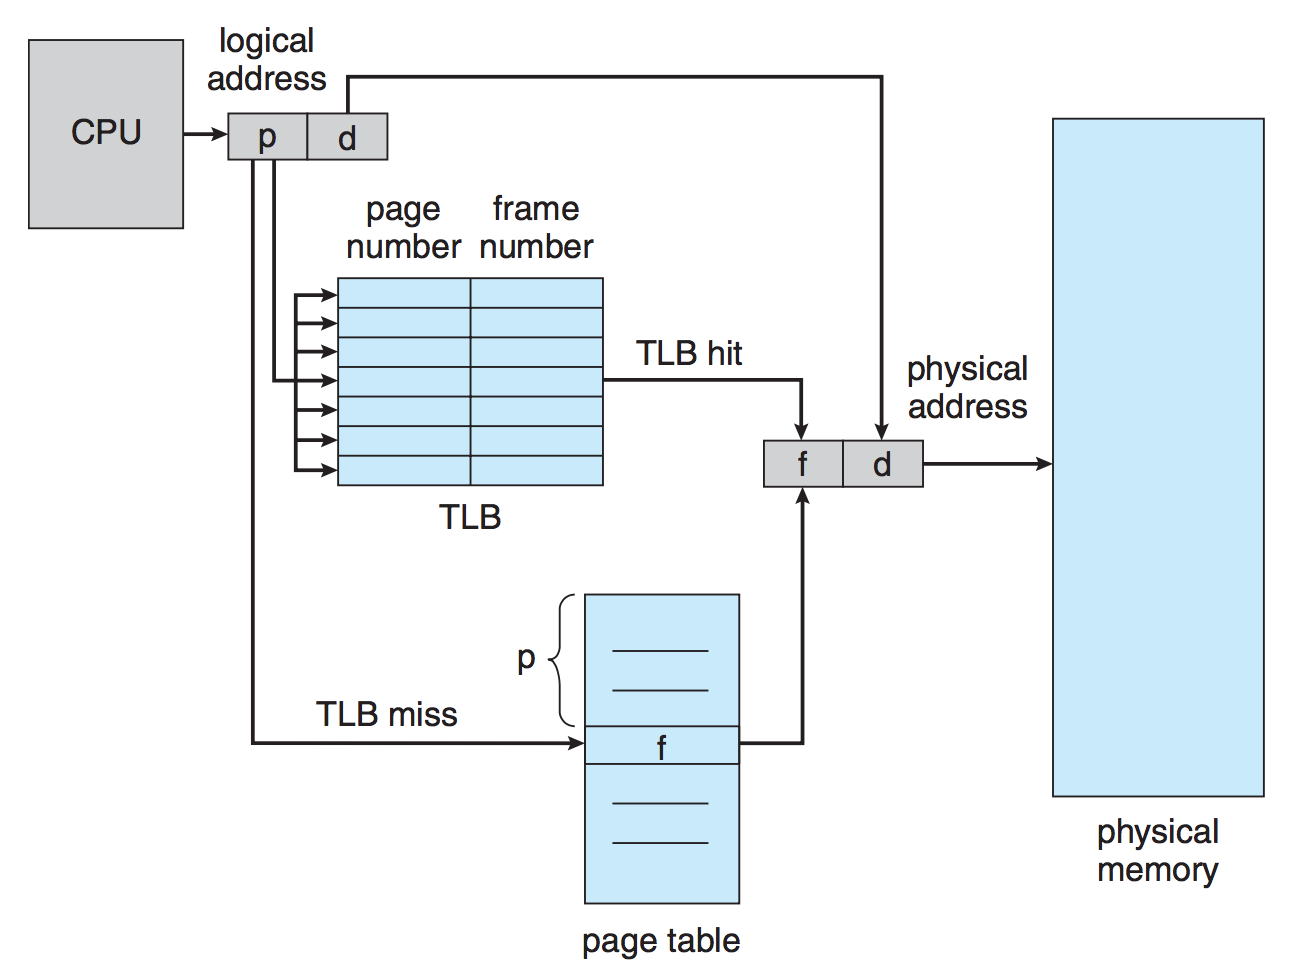
\includegraphics[width=0.65\textwidth]{images/tlb-hardware.png}\\
Mapping of logical memory to physical memory via the page table~\cite{osc}.
\end{center}

The TLB idea is a specific instance of the strategy of caching. Much earlier, when talking about the basics of computer hardware, we mentioned that memory comes at different levels and and different speeds. Caching is a critical idea in computers and operating systems. In fact, caching is such an important topic, that it will be the next topic examined.

\bibliographystyle{alpha}
\bibliography{254}


\end{document}